



% Analisou-se também o desempenho da mesma técnica aplicada a um texto contínuo extraído de artigo da Internet que descreve seis gêneros musicais brasileiros um após um outro separados em seções. Ao observar a Figura~\ref{fig:coesaolexicaTT-generos-musicais}, nota-se que os vales são mais definidos e a maioria dos segmentos coincidem ou estão próximos a segmentação de referência. A segmentação de referência possui sete segmentos que separam uma introdução do assuntos e respeitam cada uma das subseções que tratam de um gênero musical. Obtém-se nesse cenário uma eficiência maior em relação a segmentação da ata, o que sugere que textos organizados em seções podem ter melhores benefícios com técnicas baseadas em coesão léxica que as atas, onde esse fator é menos significativo.  % ou a premissa do algoritmo não é tão boa.



  % %--- ---
  % \begin{figure}[!h]
	  % \centering
	  % 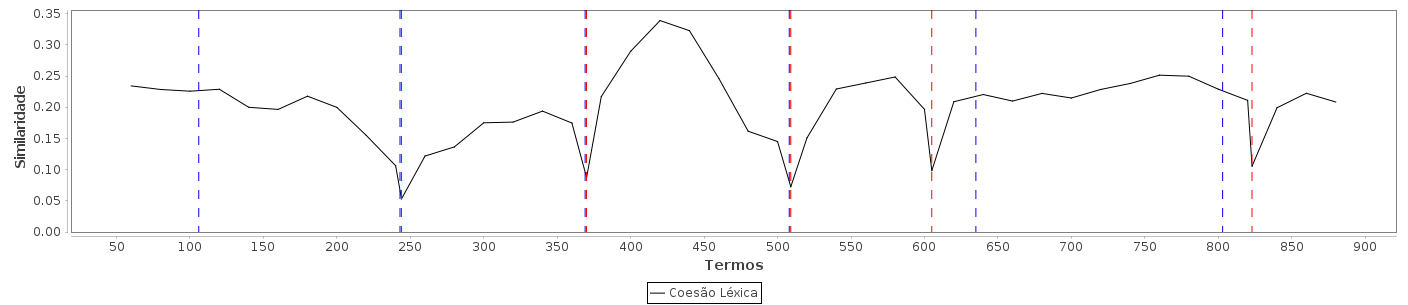
\includegraphics[width=\textwidth]{conteudo/capitulos/figs/generos-musicais-TT-40-20.png}
	  % \caption{Variação da coesão léxica ao longo de um artigo melhor estruturado em seções junto a uma segmentação automática em contraste com uma segmentação de referência.}
	  % \label{fig:coesaolexicaTT-generos-musicais}
  % \end{figure}
